\chapter{Построение математической модели объекта}
\label{ch:chap1}

\section{Вывод уравнений}

Построим математическую модель перевернутого маятника на тележке, представленного на рисунке \ref{1_pic_may}. В качестве переменных состояния выберем линейную координату тележки $a$, скорость тележки $\dot{a}$, угол отклонения маятника от вертикали $\varphi$, угловую скорость маятника $\dot{\varphi}$. В качестве управляющей переменной $u$ примем горизонтальную силу, приложенную к тележке. В качестве внешнего возмущения $f$ примем вращающий момент, действующий на маятник. В качестве выходных (измеряемых) примем величины $y_1 = a$ и $y_2 = \varphi$.

\begin{figure}[h]
\center{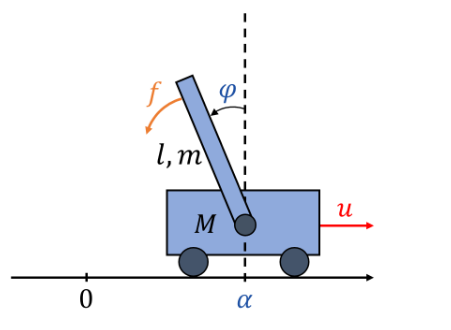
\includegraphics[width=0.8\linewidth]{pic/1_pic_may.png}}
\caption{Перевернутый маятник на тележке.}
\label{1_pic_may}
\end{figure}

Введем переменные состояния

\begin{equation}
    \begin{cases}
        x_1 = a\\
        x_2 = \dot{a}\\
        x_3 = \varphi \\
        x_4 = \dot{ \varphi}
    \end{cases}
\end{equation}

Пусть $T$ -- кинетическая энергия системы, $T_{\text{тележки}}$, $T_{\text{маятника}}$ -- кинетическая энергия тележки и маятника соответственно.

\begin{equation}
    T_{\text{тележки}} = \frac{M \dot{a}^2}{2}
\end{equation}

\begin{equation}
T_{\text{маятника}} = \frac{m}{2} \left( \dot{x}^2_{\text{маятника}} + \dot{y}^2_{\text{маятника}}  \right)  = \frac{\rho Sl}{2} \left( \dot{x}^2_{\text{маятника}} + \dot{y}^2_{\text{маятника}}  \right),
\end{equation}

где $l$ -- длина стержня, $S$ -- площадь сечения, $\rho$ -- плотность.

\begin{multline}
T_{\text{маятника}}   = \frac{\rho Sl}{2} \left( \dot{x}^2_{\text{маятника}} + \dot{y}^2_{\text{маятника}}  \right) = \\=\frac{\rho S}{2} \int \limits_0^l \left( \left( \dot{a} - \left( \lambda\sin \varphi \right)'_t \right)^2 + \left( \left(\lambda \cos \varphi \right)'_t \right)^2 \right) d \lambda =\\=
\frac{m\dot{a}^2}{2} + \frac{\rho S}{2} \int \limits_0^l \left(  -2 \lambda \dot{a} \dot {\varphi} \cos{\varphi} + \lambda^2  \dot {\varphi}^2 \cos^2\varphi +  \lambda^2 \dot{\varphi}^2 \sin^2 \varphi \right) d \lambda =\\= \frac{m\dot{a}^2}{2} + \frac{\rho S}{2} \int \limits_0^l \left(  -2 \lambda \dot{a} \dot {\varphi} \cos{\varphi} + \lambda^2  \dot {\varphi}^2  \right) d \lambda =\\= \frac{m\dot{a}^2}{2} + \frac{\rho S}{2} (-l^2 \dot{a} \dot {\varphi} \cos{\varphi} + \frac{l^3\dot {\varphi}^2}{3})  = 
\frac{m\dot{a}^2}{2} - \frac{ml \dot{a} \dot{\varphi}\cos{\varphi}}{2} + \frac{ml^2\dot {\varphi} ^2}{6}
\end{multline}


\begin{multline}
    T = T_{\text{тележки}} + T_{\text{маятника}} = 
    \frac{M \dot{a}^2}{2} + \frac{m\dot{a}^2}{2} - \frac{ml \dot{a} \dot{\varphi}\cos{\varphi}}{2} + \frac{ml^2\dot {\varphi} ^2}{6} =\\=
    \frac{(M+m) \dot{a}^2}{2} - \frac{ml\dot{a}  \dot{\varphi} \cos \varphi}{2} + \frac{ml^2 \dot{\varphi}^2}{6}
\end{multline}

Запишем систему уравнений Лагранжа

\begin{multline}
    \begin{cases}
        \frac{d}{dt} \frac{\partial T}{\partial \dot{a}} - \frac{\partial T}{\partial a} = u\\
         \frac{d}{dt} \frac{\partial T}{\partial \dot{\varphi}} - \frac{\partial T}{\partial \varphi} = f
    \end{cases} \Rightarrow 
    \begin{cases}
        \left(M+m \right) \ddot{a} - \frac{ml(\ddot{\varphi} \cos \varphi - \dot{\varphi}^2 \sin \varphi)}{2} = u\\
        \frac{ml^2 \ddot{\varphi}}{3} +\frac{ml \dot{a} \dot{\varphi} \sin \varphi}{2} - \frac{ml \ddot{a} \cos \varphi}{2} = f
    \end{cases} \Rightarrow\\ \Rightarrow
     \begin{cases}
        \left(M+m \right) \ddot{a} - \frac{ml(\ddot{\varphi} \cos \varphi - \dot{\varphi}^2 \sin \varphi)}{2} = u\\
        \frac{ml^2 \ddot{\varphi}}{3} -\frac{mgl \sin \varphi}{2} - \frac{ml \ddot{a} \cos \varphi}{2} = f
    \end{cases}
\end{multline}

Преобразуем данную систему уравнений

\begin{equation}
\begin{cases}
    \ddot{a} = - \frac{3 \cos{\varphi} \sin {\varphi} g lm + 6 \cos{\varphi}f-2 \dot{\varphi}^2\sin{\varphi}l^2m+4lu}{l(3 \cos^2 \varphi m - 4m -4M)}\\[2ex]
    \ddot{\varphi} = \frac{3(\cos \varphi \sin \varphi \dot{\varphi}^2l^2m^2-2lmu \cos{\varphi}-2glm^2 \sin{\varphi} - 2 glmM \sin{\varphi} - 4fm - 4fM)}{l^2m(3m \cos^2 \varphi -4m-4M)}
    \end{cases}
\end{equation}


\begin{equation}
\label{1_model_full}
    \begin{cases}
        \dot{x}_1 = x_2\\
        \dot{x}_2 = - \frac{3 \cos{\varphi} \sin {\varphi} g lm + 6 \cos{\varphi}f-2 \dot{\varphi}^2\sin{\varphi}l^2m+4lu}{l(3 \cos^2 \varphi m - 4m -4M)}\\
        \dot{x}_3 = x_4\\
        \dot{x}_4  = \frac{3(\cos \varphi \sin \varphi \dot{\varphi}^2l^2m^2-2lmu \cos{\varphi}-2glm^2 \sin{\varphi} - 2 glmM \sin{\varphi} - 4fm - 4fM)}{l^2m(3m \cos^2 \varphi -4m-4M)}\\
        y_1 = x_1\\
        y_2 = x_3
    \end{cases}
\end{equation}


\section{Точки равновесия}
Найдем точки равновесия системы из условия $\dot{x}_i = 0$ и $u=0$, $f = 0$

\begin{multline}
    \begin{cases}
        \dot{x}_1 = x_2 = 0\\
        \dot{x}_2 = - \frac{3 \cos{\varphi} \sin {\varphi} g lm + 0-2 \dot{\varphi}^2\sin{\varphi}l^2m+0}{l(3 \cos^2 \varphi m - 4m -4M)} = 0\\
        \dot{x}_3 = x_4 = 0\\
        \dot{x}_4  = \frac{3(\cos \varphi \sin \varphi \dot{\varphi}^2l^2m^2-0-2glm^2 \sin{\varphi} - 2 glmM \sin{\varphi} - 0 - 0)}{l^2m(3m \cos^2 \varphi -4m-4M)} = 0\\
    \end{cases} \Rightarrow \\ \Rightarrow
    \begin{cases}
        \dot{x}_1 = x_2 = \dot{a} =0\\
        \dot{x}_2 = - \frac{3 \cos{\varphi} \sin {\varphi} g lm -2 \dot{\varphi}^2\sin{\varphi}l^2m}{l(3 \cos^2 \varphi m - 4m -4M)} = 0\\
        \dot{x}_3 = x_4 = \dot{\varphi} = 0\\
        \dot{x}_4  = \frac{3(\cos \varphi \sin \varphi \dot{\varphi}^2l^2m^2-2glm^2 \sin{\varphi} - 2 glmM \sin{\varphi} )}{l^2m(3m \cos^2 \varphi -4m-4M)} = 0\\
    \end{cases} \Rightarrow \\ \Rightarrow
    \begin{cases}
        \dot{x}_2 = - \frac{3 \cos{\varphi} \sin {\varphi} g lm}{l(3 \cos^2 \varphi m - 4m -4M)} = 0\\
        \dot{x}_4  = \frac{3(-2glm^2 \sin{\varphi} - 2 glmM \sin{\varphi} )}{l^2m(3m \cos^2 \varphi -4m-4M)} = 0\\
    \end{cases} \Rightarrow
    \begin{cases}
        \cos{\varphi} \sin{\varphi} = 0\\
        m\sin{\varphi}+M \sin{\varphi} = 0
    \end{cases} \Rightarrow \\
    \Rightarrow
    \varphi = \pi k, k \in \mathbf{Z}
\end{multline}

Запишем вектор состояния для точек равновесия

\begin{equation}
    \begin{cases}
        x_1 = a \in \mathbf{R}\\
        x_2 = \dot{a} = 0\\
        x_3 = \varphi = \pi k, k \in \mathbf{Z} \\
        x_4 = \dot{\varphi} = 0
    \end{cases}
\end{equation}

\section{Линеаризация}

Линеаризуем уравнение объекта около точки равновесия $(x,u,f) = 0$ (в нашем случае -- верхнее положение маятника). При линеаризации воспользуемся следующими приемами: $\sin x \approx x$, $\cos x \approx 1$, $x^{n+1} \approx 0$ для малых $x$ и $n \in \mathbf{N}$. Будем считать $\varphi$ малым.

\begin{multline}
    \begin{cases}
        \dot{x}_1 = x_2\\
        \dot{x}_2 = - \frac{3 \cos{\varphi} \sin {\varphi} g lm + 6 \cos{\varphi}f-2 \dot{\varphi}^2\sin{\varphi}l^2m+4lu}{l(3 \cos^2 \varphi m - 4m -4M)}\\
        \dot{x}_3 = x_4\\
        \dot{x}_4  = \frac{3(\cos \varphi \sin \varphi \dot{\varphi}^2l^2m^2-2lmu \cos{\varphi}-2glm^2 \sin{\varphi} - 2 glmM \sin{\varphi} - 4fm - 4fM)}{l^2m(3m \cos^2 \varphi -4m-4M)}
    \end{cases} \Rightarrow\\
    \Rightarrow
    \begin{cases}
        \dot{x}_1 = x_2\\
        \dot{x}_2 =  \frac{3  x_3 g lm + 6 f+4lu}{l(m +4M)}\\
        \dot{x}_3 = x_4\\
        \dot{x}_4  = \frac{3( 2lmu +2glm^2 x_3 + 2 glmM x_3 + 4fm + 4fM)}{l^2m(m+4M)}
    \end{cases}  \Rightarrow\\
    \Rightarrow
    \begin{cases}
        \dot{x}_1 = x_2\\
        \dot{x}_2 =  \frac{3   g m}{m +4M}x_3 + \frac{4}{m +4M}u + \frac{6 }{l(m +4M)}f\\
        \dot{x}_3 = x_4\\
        \dot{x}_4  = \frac{6g( m  +  M  )}{l(m+4M)}x_3 + \frac{6  }{l(m+4M)}u + \frac{12(  m + M)}{l^2m(m+4M)}f
    \end{cases} 
\end{multline}

Перейдем к математической модели в виде
\begin{equation}
\label{1_model_lin}
\begin{cases}
     \dot{x} = Ax + Bu + Df,\\
     y=Cx,
\end{cases}
\end{equation}
где $A$, $B$, $C$, $D$ -- постоянные матрицы, зависящие от значений $M$, $m$, $g$, $l$. Здесь $x = (x_1, \dots , x_4)$ -- совокупный вектор состояния, $y = (y_1,  y_2)$ -- вектор измеряемых величин.

\begin{multline}
    A = \begin{bmatrix}
        0 & 1 & 0 & 0\\
        0 & 0 &  \frac{3   g m}{m +4M} & 0\\
        0 & 0 & 0 & 1\\
        0 & 0 & \frac{6g( m  +  M  )}{l(m+4M)} & 0
    \end{bmatrix}, 
    B = \begin{bmatrix}
        0\\
        \frac{4}{m +4M}\\
        0\\
        \frac{6  }{l(m+4M)}
    \end{bmatrix},\\ 
    C^T = \begin{bmatrix}
        1 & 0\\
        0 & 0\\
        0 & 1\\
        0 & 0
    \end{bmatrix}, 
    D = \begin{bmatrix}
        0\\
        \frac{6 }{l(m +4M)}\\
        0\\
        \frac{12(  m + M)}{l^2m(m+4M)}
    \end{bmatrix}
\end{multline}

\section{Выбор исходных данных}

Получим численные значения массы тележки $M=264.5866$, массы маятника $m = 9.1747$ и длины маятника $l =2.5849$. Ускорение свободного падения $g = 9.81 \, \,  \frac{\text{м}}{\text{с}^2}$.

После подстановки численных значений получим следующие матрицы системы

\begin{multline}
    A = \begin{bmatrix}
        0 & 1 & 0 & 0\\
        0 & 0 &  0.2529 & 0\\
        0 & 0 & 0 & 1\\
        0 & 0 & 5.8395 & 0
    \end{bmatrix}, 
    B = \begin{bmatrix}
        0\\
        0.0037\\
        0\\
        0.0022
    \end{bmatrix},\\ 
    C^T = \begin{bmatrix}
        1 & 0\\
        0 & 0\\
        0 & 1\\
        0 & 0
    \end{bmatrix}, 
    D = \begin{bmatrix}
        0\\
        0.0022\\
        0\\
        0.0502
    \end{bmatrix}
\end{multline}


\endinput